%%%%%%%%%%%%%%%%%%%%%%%%%%%%%%%%%
% 6CCS3PRJ Final Year Individual Project Report
% alvin.lam@kcl.ac.uk
%%%%%%%%%%%%%%%%%%%%%%%%%%%%%%%%%
\documentclass[11pt]{informatics-report}
\usepackage{color, tikz, listings, csquotes, multirow, quotchap, float, longtable}
\usepackage[square,sort,comma,numbers]{natbib} %References

%%%%%%%%%%%%%%%%%%%%%%%%%%%%%%%%%
% Front Matter - project title, name, supervisor name and date
%%%%%%%%%%%%%%%%%%%%%%%%%%%%%%%%%
\title{6CCS3PRJ Final Year\\\vspace{0.175cm}Knowledge Graph generation from diverse datasets using SPARQL Anything}
\author{Alvin Lam}
\studentID{K20045786}
\supervisor{Dr Albert Mero{\~n}o-Pe{\~n}uela}

\date{\today}

\abstractFile{FrontMatter/abstract.tex}
\ackFile{FrontMatter/acknowledgements.tex}

\begin{document}
\createFrontMatter
\onehalfspacing
\tableofcontents
\doublespacing

%%%%%%%%%%%%%%%%%%%%%%%%%%%%%%%%%
% Report Content
%%%%%%%%%%%%%%%%%%%%%%%%%%%%%%%%%
% You can write each chapter directly here or in a separate .tex file and use the include command.

% Future tense
\chapter{Introduction}
A knowledge graph is a method of representing real-world knowledge in a graphical format and is an application of knowledge engineering. The field of knowledge engineering involves designing, creating and maintaining knowledge-based systems \cite{studer_benjamins_fensel_1998}. Knowledge graphs require the creation of ontologies, which is a specification of the concept \cite{Breitman2007}. The primary aim of this project is to use the knowledge graph generation tool: SPARQL Anything and a given organ-oriented dataset to create a knowledge graph; the process in which will be detailed in this report. This first chapter will introduce the rationale, aims and scope of this project. 

\section{Rationale}
\hspace{0.5cm} There are many information sources today that are still not computationally represented or fully explored on the World Wide Web (WWW). In an article \cite{bizer2011linked}, the authors (including creator of the WWW: Tim Berners-Lee) discuss substantial amounts of structured data published on the WWW but show there is ample opportunity for further exploration of other topics. Therefore, there is demand for a means of representing information, potentially through the use of knowledge graphs, to make vast amounts of web data available for computational and human use. Finding an automated method of generating knowledge graphs from structured data or text found on the WWW is vital to addressing this demand. Current solutions for generating knowledge graphs include SPARQL-Generate \cite{sparqlgenerate}, RML \cite{rml} and Large Language Models (LLMs). LLMs are machine-learning models trained by enormous amounts of data to mimic the patterns of natural language with ChatGPT \cite{chatgptwebsite} being an example of such implementation. Nonetheless, the capability of these tools is restricted by the number of input formats they can accommodate and their level of complexity in terms of learnability \cite{sparqlanything}. Consequently, selecting SPARQL Anything \cite{sparqlanythinggithub} for implementation was most favourable. 

Generating knowledge graphs directly from datasets is not trivial as the process is complex and requires an understanding of knowledge engineering. Knowledge engineering, itself, requires experience and research in areas such as: what ontologies to create or use, what vocabularies to use and what classes to use. Thus, knowledge graph generation from a dataset is not instantaneous and requires extensive research. In the case of smaller knowledge graphs, it is possible to create knowledge graphs without the use of a tool manually. Nonetheless, physically the knowledge graph triple by triple would be time-consuming and is prone to human error, especially for larger knowledge graphs and datasets. This approach is also not sustainable. 

Motivation for organ representation, in particular, revolves around the lack of detail surrounding them. Current musical culture representation is generally insufficient \cite{polifoniaproject}, thus specific information regarding organs is necessary to enable the empowerment of such a complex structure. The organ is a fundamental part of music history and a distinguished composer- Mozart lauded the instrument as ``the king of instruments". Furthermore, Johann Sebastian Bach, a renowned composer widely regarded as one of the greatest composers of all time, had a strong preference for the organ \cite{wolff2011organs}. Enrichment of existing representations with vast amounts of detail about organs is a powerful method of honouring such a venerable instrument. The wealth of valuable information in this emerging field of organs will, therefore, enable more effective querying and strengthen its symbolic representation. 

\section{Aims}
\hspace{0.5cm} Integration of various data sources into a single, encapsulated knowledge graph can enable the sharing and understandability of this information by both humans and machines. Knowledge graphs may provide economic advantages by reducing the time and effort to analyse vast amounts of data. Consumers may use the knowledge graphs for their own needs or follow the process outlined in the report to create their own knowledge graphs.

To the extent of our research, creating knowledge graphs for this particular subject (organs) had not yet been fully explored in this level of detail. For instance, knowledge graphs were previously developed for music recommendation systems \cite{oramas2016sound} by other researchers. So knowledge graph generation techniques had been done previously, but the employed methodology is of a different context to our problem. Existing organ knowledge graphs on Wikidata \cite{organwikidata}, MusicBrainz \cite{organmusicbrainz} and DBpedia \cite{organdbpedia} are sufficient for basic familiarity, but do not go into the same amount of depth as the knowledge graph created in this project. This project also aims to address this particular knowledge representation gap. 

\section{Scope}
\hspace{0.5cm} The project is part of the Polifonia project, which seeks to create an ecosystem of computational tools and methodologies to spread knowledge about musical history on the internet \cite{polifoniaproject}. Therefore, this report assists the Polifonia project in achieving its objectives and facilitates its progression. This designated project involves a dataset centred around organs so the report includes a breakdown of the various organ components as well as background information regarding technical knowledge. 

This report will detail the process of knowledge graph generation using an organ-orientated dataset and ontology \cite{organontology}, both of which are contextualised to understand the dataset fully and to refine the provided ontology. In order to commence, knowledge of the semantic web and its capabilities are required so as to understand the scope of the project. Researching and being able to interpret RDF (a standard model for data interchange on the web \cite{gottschalk2021creation} used for representing and exchanging metadata), ontologies and knowledge graphs is also required to reach the solution as well as interpret it. 

The following chapters provide a comprehensive view of the design and implementation process for generating knowledge graphs. The \textit{Design} chapter complements the implementation phase by using visual tools and careful planning through software development techniques. Subsequently, the \textit{Implementation} chapter meticulously explains the steps required to reach the final solution. A thorough evaluation of the produced knowledge graph is performed with both qualitative and quantitative forms of assessment being carried out. The legal, social, ethical and professional issues surrounding this project are also reviewed to ensure adherence to the Code of Conduct \& Code of Good Practice issued by the British Computer Society \cite{bcs} as well as the FAIR Principles \cite{fairprinciples}. This is also intended to assist in identifying any potential issues that may arise during the project.

Finally, the conclusion summarises work completed during the course of this project and includes a discussion on future work and limitations. 

\usetikzlibrary {arrows}
\usetikzlibrary {shapes.geometric}
\usetikzlibrary {patterns}

\chapter{Background}
First, background of this project is discussed and suitable explanations provide context for the entire project. The broad scope of the project is presented before going into project-specific details in the \textit{Context} chapter.

\section{The Semantic Web}
\hspace*{0.5cm} The Semantic Web is an extension of the World Wide Web (WWW) that allows information on it to be machine-readable \cite{semanticweb}. The concept was founded by Tim Berners-Lee (founder of the WWW) with the idea that machines can easily interpret information available on the WWW. Tim Berners-Lee initially thought of this idea in 1999 stating ``I have a dream for the Web [in which computers] become capable of analysing all the data on the Web – the content, links, and transactions between people and computers. A `Semantic Web'" \cite{berners-TBLBook}. Ultimately, the semantic web aims to empower the knowledge embedded online so that it can be parsed by machines \cite{semanticweb}. 

An example of these developments can be seen in a data storage project that contains structures interpretable by both humans and machines- Wikidata. Wikidata is a large open knowledge base that is part of the Wikimedia family (including Wikipedia) and is connected to other datasets as well \cite{wikidata}. Data is stored in WikiData using various web data storage methods such as JSON, XML and RDF (Resource Description Framework). The latter is described in more detail in the next section.  

Another example within the project scope is MusicBrainz. MusicBrainz also provides information that is stored using RDF \cite{musicbrainz}. In this case, MusicBrainz's focus is around music so it may be more relevant and provide more specific data for the project. 

\subsection{Resource Description Framework}
\hspace*{0.5cm} Resource Description Framework (RDF) is a method in which data can be stored, similar to how data can be stored in JSON or XML formats. However, the structure of RDF is very different. The general idea of RDF revolves around the concept of linked and connected data so RDF stores data in triples with relationships between data. Data stored in this format is both machine and human-readable, making the reuse and extension of data semantics possible \cite{rdf}. Each triple follows this structure: 

\vspace{-0.1cm}
\begin{center}
\begin{displayquote}
   \textit{subject predicate object}
\end{displayquote} 
\end{center}
\vspace{-0.2cm}

\textbf{Subject:} \\
The subject is the entity that the triple is about or refers to, which is typically a resource. A resource can be a Uniform Resource Identifier (URI- a string that identifies a name or resource on the Internet \cite{sikos_2015}), a physical thing or an abstract concept. 

\textbf{Predicate:} \\
The predicate conveys the relationship between subject and object (i.e. how they are related). 

\textbf{Object:} \\
The object is an entity that the triple describes in relation to the subject. This can also be blank. 

In this project, we will look closer at the Turtle (TTL) format for RDF. A TTL file represents RDF triples with a subject, object and relationship. This format is specifically relevant when representing multiple related RDF triples (RDF Graph) and allows them to be readable by both humans and machines \cite{TTL}.

An example of an RDF statement (in TTL) can be seen below:

\vspace{-0.4cm}
\begin{center}
\lstset
{
    breaklines=true,
    breakatwhitespace=true,
    basicstyle=\linespread{1.5}\ttfamily,
}
\begin{lstlisting}
    <http://www.example.com/Alvin> 
    <http://www.example.com/vocab#studiesAt> 
    <http://www.example.com/KCL>
\end{lstlisting}
\end{center} 
\vspace{-0.3cm}

\noindent In this example, 
\vspace{-0.15cm}
\begin{itemize}
    \itemsep0em 
\item \textbf{The subject is:} \\ \textit{``http://www.example.com/Alvin"}
\item \textbf{The predicate is:} \\ \textit{``http://www.example.com/vocab\#studiesAt"}
\item \textbf{The object is:} \\ \textit{``http://www.example.com/KCL"}
\end{itemize}
\vspace{-0.1cm}

This statement indicates that the entity \textit{``http://www.example.com/Alvin"} studies at the entity \textit{``http://www.example.com/KCL"}, according to the vocabulary defined by \\\textit{``http://www.example.com/vocab"}. However, writing all the various URI links separately is tedious and can look confusing for the human reader so using prefixes as shown below can make it more concise:

\vspace{-0.2cm}
\lstset
{
    breaklines=true,
    breakatwhitespace=true,
    basicstyle=\linespread{1.5}\ttfamily,
}
\begin{center}
\begin{lstlisting}
    @prefix ex: <http://www.example.com/>. 
    @prefix exVocab: <http://www.example.com/vocab#>. 

    ex:Alvin exVocab:studiesAt ex:KCL
\end{lstlisting}
\end{center} 
\vspace{-0.2cm}

This example uses two abbreviations of URIs and has named the alias for these URIs to be `ex' and `exVocab' respectively, simplifying the triple. 

An English translation of the RDF triple is written below: 

\vspace{-0.1cm}
\begin{center}
    \textit{``Alvin studies at KCL".}
\end{center}
\vspace{-0.1cm}

As mentioned previously, RDFs can also be visualised in graph format with numerous relationships between subjects and objects, specifying their relationships. In particular, this project's produced knowledge graph will be in RDF format and be represented in a TTL file. RDFs can be used to describe ontologies, which are described in the next section.

\section{Ontology}
\hspace{0.5cm} An ontology is a conceptual framework for modelling domain knowledge \cite{ontology}. Ontologies make use of RDF triples by having two nodes (the subject and predicate) and an edge (the relationship). They act as models in which real data can be input, so these ontologies can be reused in different contexts and shared between users. These generalised models are ideal for knowledge graph generation because data from different contexts can be displayed in the same way using the same ontology. 

The main components of an ontology are similar to the RDF triples in the previous section but have different names. They involve:

\vspace{-0.15cm}
\begin{itemize}
    \itemsep0em 
\item \textbf{Classes}: \\
A collection of objects or things that are related to each other in some way.

\item \textbf{Relationship}: \\
A link between a class and an attribute that describe how they are related. 

\item \textbf{Attributes}:\\ 
A characteristic or property that a class may have, which is described by the relationship between them.

\end{itemize}
\vspace{-0.15cm}

In relation to RDF statements, a connection between two nodes in an ontology will have subject and object nodes with a connecting edge specified by the predicate. \textit{Figure 2.1}, is an example of a graphical visualisation in the context of a football team:

\begin{figure}[H]
\begin{center}
    \begin{tikzpicture} [
        circle/.style={draw=brown, ellipse, ultra thick, fill=brown!30},
        square/.style={draw=brown, rectangle, ultra thick, fill=brown!30},
        align=center,
        node distance=5cm ]
    \node[circle] (q1)  {Football Team};
    \node[circle, right of=q1] (q2)  {Captain};
    \draw (q1) edge[->,above] node {\tt hasCaptain} (q2);
    \node[square, above of=q1] (q3) {Year};
    \draw (q1) edge[->,left] node {\tt foundedYear} (q3);
    \node[circle, above of=q2] (q3) {Manager};
    \draw (q1) edge[->,right] node {\tt hasManager} (q3);
    \draw (q3) edge[->,right] node {\tt selectsCaptain} (q2);
    \end{tikzpicture}
\end{center}
\vspace{-0.2cm}
\caption{Example Arsenal Ontology}
\end{figure}
\vspace{-0.15cm}

\textit{Figure 2.1} depicts a Football Team with a Manager and a Captain. The Manager and Captain (of the football team) also have a relationship because the manager selects a specific captain for the football team. The attribute `Year' only describes the `Football Team' class so is denoted as such.

Ontologies are the framework in which knowledge graphs can be constructed and guide the generation of knowledge graphs. 

\subsection{Knowledge Graphs}
\hspace{0.5cm} A knowledge graph is a graph (i.e. data graph) that depicts real-world knowledge or data \cite{knowledgegraph}. Similar to ontologies, knowledge graphs are often represented as a network of interconnected nodes and edges but instead, nodes represent real-world entities (such as people or places) and edges represent the real-world relationships between them (such as `owns' or `discovered'). 

As mentioned, knowledge graphs apply real data from an ontology framework. With a dataset and relevant ontology, we can create specific instances of each ontological relationship. 

Knowledge graphs are used in a variety of real-world applications including search engines, recommendation systems and natural language processors. More detail on these examples are below:

\vspace{-0.1cm}
\begin{itemize}
\itemsep0em 
\item \textbf{Search Engines:} \\Knowledge graphs are used by search engines such as Google to find appropriate results given a search query. Results are interpreted and relevant information is displayed based on relationships between the URIs and meaning of the search term. The most relevant information with regard to the search query is displayed to the user. The method in which a knowledge graph aids a specific search query is called a ``semantic search" and provides more accurate and relevant results. This mirrors how humans tend to think by emulating our natural ability to find associations between data \cite{searchengine}.  

\item \textbf{Recommendation Systems:} \\Knowledge graphs can be used in such systems because there are often many associations between different entities. Recommendation systems use relationships in the knowledge graph to display the most relevant data to the user. 

\item \textbf{Natural Language Processing:}\\ In this context, knowledge graphs are used to establish connections between distinct terms linked within text. A system employing Natural Language Processing may want to understand the meaning of a sentence and be able to interpret and input it into a search query so that relevant results can be found. 
\end{itemize}

An example of a knowledge graph can be in \textit{Figure 2.2}, following the ontology in \textit{Figure 2.1} displayed in the ontology section above:

\begin{figure}[H]
\begin{center}
    \begin{tikzpicture} [
        circle/.style={draw=red, ellipse, ultra thick, fill=red!30},
        square/.style={draw=red, rectangle, ultra thick, fill=red!30},
        align=center,
        node distance=5cm ]
    \node[circle] (q1)  {Arsenal};
    \node[circle, right of=q1] (q2)  {Ødegaard};
    \draw (q1) edge[->,above] node {\tt hasCaptain} (q2);
    \node[square, above of=q1] (q3) {1886};
    \draw (q1) edge[->,left] node {\tt foundedYear} (q3);
    \node[circle, above of=q2] (q3) {Arteta};
    \draw (q1) edge[->,left] node {\tt hasManager} (q3);
    \draw (q3) edge[->,right] node {\tt selectsCaptain} (q2);
    \end{tikzpicture}
\end{center}
\vspace{-0.4cm}
\caption{Example Arsenal Knowledge Graph}
\end{figure}
\vspace{-0.1cm}

\textit{Figure 2.2} describes Arsenal's men's football team. Arteta is the manager of Arsenal and Arsenal's captain is Ødegaard. Arteta (the manager) also selects the captain. The year Arsenal was founded is displayed in the graph as 1886.

The more linked data we add from the dataset, the larger the knowledge graph will grow.

\section{SPARQL}
\hspace{0.5cm} SPARQL enables us to query RDF data formats and retrieve specific data from large RDF files. SPARQL queries often have the same structure as standard SQL queries. Specific data can be specified and filtered by stating the subject, object and relationship in the query's SELECT and WHERE clause respectively \cite{sparlbook}. An example of a SPARQL Query is shown with an explanation below:

\begin{lstlisting}
PREFIX foaf: <http://xmlns.com/foaf/0.1/>
SELECT ?first_name 
       ?surname
WHERE
  {
    ?person  a          foaf:Person.
    ?person  foaf:name  ?first_name.
    ?person  foaf:surname  ?surname.
  }
\end{lstlisting}
\textit{Example from}: \cite{foaf}

\medskip
Here, the shortcut `foaf' (friend of a friend) is used, which is often used to describe people, their characteristics, relationships and other information about them \cite{foaf}.

The \textbf{SELECT} part of the query extracts all the first and last names of people in the queried TTL file with RDF type \textit{foaf:Person}. The selected people must also have a name and surname specified in the file.

The \textbf{WHERE} clause of the query specifies that the queried variable \textit{?person} belongs to the RDF class \textit{foaf:Person}. The \textit{?person} should also possess both a name and a surname represented by the property \textit{foaf:name} and \textit{foaf:surname} respectively.

In conclusion, if the query were to be executed in an appropriate RDF document, the result would display the first and last names of all individuals in the TTL file of type \textit{foaf:Person}. Moreover, the individuals outputted will have both a name and surname property.

\chapter{Context}
In this chapter, I will detail the context of my dataset and project. I have provided an explanation of all the relevant information included in my dataset or classes included in the organ dataset. I also gave a brief introduction to the tool I will be using to complete this project: SPARQL-Anything. 

\section{Organs}
\hspace{0.5cm} The dataset that has been provided revolves around the musical instrument: Organs. Mozart once described organs as:

\begin{quote}
    \textit{"The king of instruments."}
\end{quote}

An organ can come in various different sizes ranging from the size of a small upright piano to a large structure consisting of many sub-systems. In the following chapter, I will provide a description of this instrument.

\subsection{A Brief History}
\hspace{0.5cm} 
The inventor of the organ is accredited by many sources to an engineer in Alexandria in the third century BC called Ctesibius. In the first century AD, organs used water and hydraulic engineering to generate sound. \cite{organhistory}

During the 14th century, organs had evolved from just the use of pedals and saw the development of a keyboard so a larger range of sounds could be made. This was accommodated with the creation of new pipes so having access to play more of these unique sounds was beneficial. These organs laid the building blocks for the organs we recognise today. \cite{organmedivalhistory}

Due to the modernisation of the world, creation of organs has become a lot easier allowing them to become more complex. Recent organ builders have had access to a plethora of materials and tools required to create these large structures with complex systems. Being able to study and explore different types of organs with ease, also aided the development of such structures.  \cite{organhistory1}

\noindent \subsection{How Organs Work:}
\hspace{0.5cm} Operation of the organ involves generating and directing airflow to the requested pipe this, in turn, sound is produced when these pipes vibrate. The organist uses the keyboard and pedals to control the flow of air to pipes and draws stops to combine different sets of pipes to produce unique, blended sounds.  \cite{organvideo}

\noindent Generally, the organ system works as follows:
\begin{enumerate}
\item Note is played on keyboard.
\item Pressurised air is passed through organ system.
\item When a particular stop is pulled, an internal slider is moved allowing air to pass through pipes.
\item Sound for that particular key and stop is produced.
\end{enumerate}

\noindent \textbf{Pipe Types:}
\begin{itemize}
\item \underline{Reed Pipes}: Passes air through a reed (similar to a clarinet).
\item \underline{Flue Pipes}: Forces air through a pipe (similar to recorder).
\end{itemize}
\cite{organvideo}

\noindent \textbf{Stops:}
\\ \hspace*{0.5cm}Drawing/selecting a stop gives the player access to that stop's set of pipes available (for a particular key on the keyboard). 
\begin{itemize}
\item Draw Stops
\item Tabs
\end{itemize}

Multiple stops can be drawn at once in the same division and multiple pipes will produce sound (pressurised air will be passed through them) from the press of one key. \cite{organvideo}

\medskip
\noindent \textbf{Rank:}
\\ \hspace*{0.5cm} A rank is a row of pipes (controlled by a single stop) that is part of the organ which makes the same musical sound but does so at different pitches. 

For example, a rank of spire flue pipes all produce the same wind instrument sound, but each key pressed will produce a different flue pitch.  \cite{organvideo}

\medskip
\noindent \textbf{Divisions:}
\\ \hspace*{0.5cm} An organ division is a set of pipes found within an organ that are controlled by a keyboard or the pedals. Stops of an organ are arranged into divisions, which are usually given unique names. For example, some divisions include:
\begin{itemize}
\item Swell (smaller pipes).
\item Great (larger pipes).
\item Pedal.
\item Choir.
\item Positiv
\end{itemize}

All of these divisions usually accompany whatever is deemed appropriate for the given context. For example, if you are accompanying a choir, using the choir division would be best so as to not drown out the voices of the choir.  \cite{organvideo}

\medskip
\noindent \textbf{Coupler:}
\\ \hspace*{0.5cm} A coupler allows the stops of one division to be played from the keyboard of another division- the combining of divisions. For example, the "Great" division is usually played on the manual (keyboard) of the organ, but pulling the "Great to Pedal" coupler can allow for this division to be played on the pedals.

It is worth noting that couplers may look like stops and need to be pulled to be activated, but are not stops. \cite{organvideo}

\medskip
\noindent \textbf{Wind System:}
\\ \hspace*{0.5cm} Wind systems are responsible for:
\begin{itemize}
\item Producing
\item Storing
\item Delivering
\end{itemize}
the air within the organ system.

The organ wind system is a subsystem of the organ, which is responsible for delivering air to the organ's different pipes. Wind is generated within the system and then directed through a series of channels to the pipes of the organ. Upon delivery of air to each individual pipe, a sound is made based on the key or pedal pressed. \cite{organvideo}

\subsection{Organ Ontology}
\hspace{0.5cm} The organ ontology provided the framework of the knowledge graph I am going to create using the organ dataset. This covers the dataset as well as other details about an organ so that all the data can be displayed in the form of a knowledge graph, following the structure of the ontology. 

The ontology includes classes for the organ system:
\begin{itemize}
\item Organ Console
\item Organ Wind System
\item Organ Case
\item Organ Action
\item Organ Division
\end{itemize}

But the ontology also includes classes about a particular organ's owner and offers background on a given organ. For example:
\begin{itemize}
\item Description
\item Agent and the role of this agent (owner, organist, builder etc.)
\end{itemize}

\section{Polifonia Project}
\hspace{0.5cm} The Polifonia project is a European project funded by the EU Horizon 2020 Programme that will manifest the connections between musical heritage from the 16th century to the present day \cite{polifonia}. The project involves many different types of experts from musicologist to computer scientists to attempt to find links between different parts of musical cultural heritage. 

The main aim of this project is to combine computational tools and methods to access and manipulate musical cultural heritage on the WWW. Another aim is to use these computational methods in a different context (independent of Computer Science field) and test whether such techniques can be adequately applied elsewhere. Hence, the involvement of experts from all over Europe to guide the progress of this project. \cite{polifoniaproject}

The section my project is involved in is the creation of a knowledge graph in the context of pipe organs. The dataset was provided and previously put into an organised format by a musicologist as part of this project. The general organ ontology was also created prior to my project commence but requires refinement and some changes in order to create the knowledge graph. Due to the project being European-based, the data stored in the dataset is in Dutch and the knowledge graph created will also produce dutch text or terms.  

\subsection{Organ Dataset}
\hspace{0.5cm} The organ dataset provided describes the various specifics about a given organ. The dataset itself is split into many different folders and it groups specific details about an organ in one .JSON file. Each .JSON file contains information about many different organs, which can be uniquely identified by their unique id. The structure of the .JSON files follow the same format: an organs and the corresponding details about each organ in the form of a .JSON. An example of two files "base.json" and "history\_base.json" can be seen below. 

\begin{lstlisting}
    # base.json extract
    {
      "Part01_001MIDDE": {                             # Unique Organ Code
        "building": "Koorkerk",                        # Basic organ details
        "monumentnumber": "28671",
        "name": "Middelburg, Koorkerk",
        "organnumber": "971",
        "place": "Middelburg",
        "whichorgan": "",
        "year": "1479"
      },
      "Part01_002UTREJ": {
        "building": "Jacobikerk",
        "monumentnumber": "36148",
        "name": "Utrecht, Jacobikerk",
        "organnumber": "1514",
        "place": "Utrecht",
        "whichorgan": "",
        "year": "1509"
      },
      ... # Other organs
    }

    #history_base.json extract
    {
      "Part01_001MIDDE": {                              # Unique Organ Code
        "builder": "Peter Gerritsz",                    # Basic history of organ
        "originallocation": "Utrecht, Nicolaikerk",
        "year": "1479"
      },
      "Part01_002UTREJ": {
        "builder": "Gerrit Petersz",
        "originallocation": "",
        "year": "1509"
      },
      ... # Other organs
    }
\end{lstlisting}

The data is split into two different files and the unique organ name, with it's grouped relevant data, appear.  

\section{SPARQL Anything}
\hspace{0.5cm} SPARQL Anything acts as an extension of SPARQL and allows knowledge graphs to be generated from a dataset. SPARQL Anything uses Facade-X, which is similar to the Facade design pattern. The facade design pattern is a useful way to improve the usability of a complex system by providing a simpler and more intuitive interface to it. In this case, SPARQL Anything masks the complex components by allowing the user to continue to use SPARQL syntax. Using SPARQL Anything, the SERVICE operator can  be overridden and we can use SPARQL Anything within a query. \cite{sparqlanything}

The CONSTRUCT operator allows knowledge graphs to be generated, through the framework of a given ontology. \cite{sparqlanythinggithub}

SPARQL Anything allows us to query a dataset to suit our needs and generate a knowledge graph using an ontology framework all in one tool. \cite{sparqlanythinggithub}

\section{Other Tools}

\hspace{0.5cm} In this section, I will detail another way of generating knowledge graphs, in the context of organs, describing the approach as well as the positives and negatives of the suggested approach.

\subsubsection{ChatGPT}
\hspace{0.5cm}  ChatGPT is a machine-learning-based tool developed by OpenAI and is an interactive chatbot. Answers provided by the chatGPT are in a conversational manner so answers are easy to understand and are suggested to be the best chatbot to date. \cite{chatgpt} This OpenAi released a prototype chatbot on 30th November 2022 and is currently free to use. Uses of ChatGPT include:
\begin{itemize}
\item Solving programming questions.
\item Fixing bugs in code.
\end{itemize}

When ChatGPT is asked to create a knowledge graph regarding organs, this is what it produced:

\lstset
{
    breaklines=true,
    breakatwhitespace=true,
}
\begin{lstlisting}
    Nodes: Keyboard, Pedals, Pipes, Blower, Stops
    Edges:
        -  The keyboard is connected to the pipes, indicating that pressing keys on the keyboard causes the corresponding pipes to produce sound.
        -  The pedals are connected to the pipes, indicating that pressing the pedals can also cause certain pipes to produce sound.
        -  The blower is connected to the pipes, indicating that the blower supplies air to the pipes, allowing them to produce sound.
        -  The stops are connected to the pipes, indicating that the stops control which pipes are active and can produce sound.
\end{lstlisting}

This response represents a small knowledge graph mainly comprised of organ parts and how it produces sound. The output of the knowledge graph is in plain text so has to be manually read and interpreted, so is not in a machine-readable format. 

This approach is a very straightforward technique for generating an organ-related knowledge graph and makes use of the strengths of ChatGPT. The knowledge graph, although in prose, is very useful and easy to understand due to ChatGPT's ability to communicate conversationally. The information provided is based on the chatbot's general understanding of the organ and is consistent with the instrument's details. The nodes and edges in the graph that are stated in the knowledge graph are also consistent with the general information regarding an organ. 

However, this approach generates a small knowledge graph and has to be interpreted correctly in prose. In terms of the produced knowledge graph's validity, the knowledge graph does not include any real-world data, but more general topics regarding organs so the generated knowledge graph is a lot closer to an ontology than a real-world knowledge graph. The limitations of ChatGPT include that it is restricted to it's input domain \cite{chatgptwebsite}, so real-world data can not be found and passed into this ontology to create a suitable knowledge graph. 

In conclusion, the knowledge graph produced by ChatGPT is closer to an ontology about organs. The limitations surrounding ChatGPT do confine it to providing a generic solution, but if it can evolve to find a way to gather real-world data online using the Semantic Web, for instance, the knowledge graph created would be a viable solution (given the provided ontology).

\subsubsection{SPARQL-Generate and RML}
\hspace{0.5cm} Other solutions similar to SPARQL Anything's approach and implementation include: SPARQL-Generate and RML. But, the reasoning for selecting SPARQL-Anything will be detailed below.

SPARQL-Generate and RML do not support Metadata or Embedded data formats. \cite{sparqlanything} SPARQL Anything allows more flexibility during implementation and has a broader scope. 

SPARQL-Generate is an extension of SPARQL so requires the studying of the newly created extension. RML requires a mapping to RDF using a new R2RML vocabulary, so again requires studying a new language. SPARQL Anything, on the other hand, because it uses Facade-X, is reliant on SPARQL 1.1 knowledge. \cite{sparqlanything} This results in less time spent studying something completely new and easier learnability.
\chapter{Literature Review}
In this chapter, I will include any websites, papers, videos or textbooks I reviewed to help me in this project. The literature I studied covered a broad range of topics and grouped them into categories below. 

\section{Semantic Web}
\hspace{0.5cm} This section mainly involves websites, which I used for background research on different aspects of the semantic web.

\begin{itemize}
\item https://en.wikipedia.org/wiki/Semantic\_Web 
\item https://www.w3.org/standards/semanticweb/ 
\item https://en.wikipedia.org/wiki/Linked\_data
\item https://www.w3.org/RDF/
\item https://en.wikipedia.org/wiki/Resource\_Description\_Framework
\item http://xmlns.com/foaf/0.1/
\item https://en.wikipedia.org/wiki/FOAF
\item Resource Description Framework (RDF), Peter Loshin, February 2022
\item Wikidata: a new platform for collaborative data collection, April 2012, Denny Vrandečić
\end{itemize}


\section{Ontology and Knowledge Graphs}
\hspace{0.5cm} This section involves website links to help me understand what ontologies were and how they related to knowledge graphs. Researching them individually helped me gain context for the knowledge graph generation this project is about. 

\begin{itemize}
\item https://enterprise-knowledge.com/whats-the-difference-between-an-ontology-and-a-knowledge-graph/ 
\item https://www.ontotext.com/knowledgehub/fundamentals/what-are-ontologies/
\item https://en.wikipedia.org/wiki/Knowledge\_graph 
\end{itemize}


\section{Organs}
\hspace{0.5cm} This section provides context for the dataset, which is about organs. Understanding the different terms used in the dataset as well as the classes in the organ ontology was facilitated using the resources below. More websites had to be used in order to fully understand each class in the organ ontology, but the videos provided a great foundation. 

\begin{itemize}
\item https://en.wikipedia.org/wiki/Pipe\_organ 
\item https://youtu.be/4S6BErQs-HE 
\item https://youtu.be/kAlj3CE-7mM 
\item https://organhistoricalsociety.org/OrganHistory/works/works09.htm
\item https://www.britannica.com/art/organ-musical-instrument
\item https://organhistoricalsociety.org/OrganHistory/history/hist001.htm
\end{itemize}

\section{SPARQL-Anything}
\hspace{0.5cm} This section contains anything I used to help construct my query. Includes a SPARQL textbook as it familiarised me with the syntax used. 

\begin{itemize}
\item https://github.com/SPARQL-Anything/sparql.anything 
\item https://www.w3.org/TR/rdf-sparql-query/
\item Learning SPARQL 2ed: Querying and Updating with Sparql 1.1, August 2013, Bob DuCharme
\item https://arxiv.org/pdf/2106.02361.pdf
\end{itemize}

\section{Knowledge Graph Evaluation}
\hspace{0.5cm} This section contains the resources I used to discover how to critique and evaluate my completed knowledge graph. 
\begin{itemize}
\item https://www.emse.fr/~zimmermann/KGBook/Multifile/quality-assessment/
\item A Practical Framework for Evaluating the Quality of Knowledge Graphs - Haihua Chen, Gaohui Cao, Junhua Ding, Jiangping Chen (Jan 2019)
\end{itemize}

\chapter{Requirements}
In this chapter, the requirements for this project will be stated. 

\section{Preliminaries}
\hspace{0.5cm} These detailed the tools required for commencing implementation.
\begin{enumerate}
\item Installation of SPARQL Anything from \cite{sparqlanythinggithub} by downloading .jar file.
\item Installation of Java Virtual Machine on the computer. 
\item Access to a Command Line Interface.
\item A Integrated Development Environment.
\end{enumerate}

\section{Software Requirements}
\hspace{0.5cm} These requirements are centered towards what needs to be implemented and produced upon completion. Assessing and validating the solution is also necessary to ensure correctness.
\begin{enumerate}
\item Ontology must be correctly configured and input into SPARQL-Anything CONSTRUCT operator.
\item Knowledge graph created must correctly reflect the organ dataset and follow ontology structure.
\item Dataset must be refined to ensure correct data is being input into the knowledge graph.
\item Knowledge graph must expand on the current dataset using external links.
\item Knowledge graph must be evaluated to prove correctness and validity.
\item Speed of knowledge graph generation must be assessed.
\end{enumerate}

\section{User Requirements}
\hspace{0.5cm} These requirements specify what an external user should be able to do when using my solution.
\begin{enumerate}
\item User must be able to execute written query.
\item User must be able to select an organ to view information on. 
\item User must be able to see the knowledge graph after the query is executed.
\item User must be able to see relevant data in the knowledge graph.
\item User must be able to view other relevant external data in the knowledge graph.
\end{enumerate}


\chapter{Specification}
This chapter will go into more detail regarding each of the requirements specified in the previous chapter. More specifically, this chapter will provide an explanation of how each requirement can be achieved.

\section{Software Requirement Specification}
\begin{longtable}{|p{2.25cm}|p{4.5cm}|p{6.5cm}|}
\hline
\textbf{Requirement No.} & \textbf{Requirement} & \textbf{Specification}\\
\hline

1& 
Ontology must be correctly configured and input into the query's CONSTRUCT clause. &
Organ ontology created will match data from the given dataset and only relevant segments of the provided ontology will be included. To ensure the generation of a valid knowledge graph, it is important to extract relevant parts of the ontology and define the correct types. This guarantees that all classes are properly converted and ensures all relationships are accounted for with no redundant details. \\
\hline

2&
The knowledge graph created must correctly reflect the organ dataset and follow ontology structure. &
Identify data from the dataset in the knowledge graph and ensure relationships are consistent. Compare ontology with produced knowledge graph and ensure the framework is being followed. Override the SERVICE keyword in the query to use services of SPARQL Anything. \\
\hline

3&
The dataset must be refined to ensure correct data is being input into the knowledge graph. &
Query correctly navigates through the dataset to find the right data to add to the knowledge graph. This can be done through string manipulation in the query to generate the correct path, thus obtaining the right data. In the WHERE clause of the query, ensure data being input into the knowledge graph is understandable and concise (if not already).  \\
\hline

4&
The knowledge graph must expand on the current dataset using external links. &
Search for external links to expand the knowledge graph beyond the dataset and present additional relevant information. Use web resources such as WikiData, MusicBrainz and DBpedia to find potential expansion points of the knowledge graph derived from the organ dataset. Use multiple SERVICE calls (within the WHERE clause) to obtain external data and add it to the current knowledge graph. String manipulation and string-to-link conversion (IRI) may be necessary to add external links. \\
\hline

5&
Knowledge graphs must be evaluated to prove correctness and validity. &
Validate correctness of the knowledge graph produced. Look into accuracy, coverage and coherency of the produced knowledge graph and analyse the different aspects of those areas in more detail. \cite{knowledgegraphevaulationbook} and \cite{evaluationpaper}, identified in the \textit{Literature Review} Chapter, will be used to help during evaluation. \\ 
\hline

6&
Scalability of knowledge graph generation must be assessed. &
Assess speed of the query for knowledge graph generation to ensure expansion of the knowledge graph is possible in the future without encountering severe time constraints. This will measure scalability based on many different factors (more detail in the \textit{Evaluation} chapter). 
\\ \hline
\caption{Software Requirement Specification Table}
\end{longtable}

\begin{table}[!ht]
\section{User Requirement Specification}
\begin{center}
\begin{tabular}{c|p{2in}p{2.55in}}
Requirement \\ No.&Requirement&Specification\\\hline 

1&
User must be able to execute written query. & 
Upon downloading the GitHub repository and the SPARQL Anything executable, a user should be able to execute the query using SPARQL Anything and have it produce a knowledge graph. \\
\hline

2& 
User must be able to select an organ to view information on. &
When writing the command on the command line to execute the query, the user can be able to input an organ that they want to view specific information on by passing it as a parameter. The resulting knowledge graph is then specific to the requested organ. \\
\hline

3&
User must be able to see the knowledge graph following query execution. &
Upon executing the query, a knowledge graph should be visible in the form of a TTL file. The user can also see the knowledge graph on command line if they wish.\\
\hline

4&
User must be able to see relevant data in the knowledge graph. & 
The knowledge graph must display the correct data and relationships between them. When viewing the final solution, the user can compare data from the dataset and knowledge graph. Organ-specific data can be seen for the requested organ.\\
\hline

5&
User must be able to view other relevant external data in the knowledge graph. & 
The user should be able to view external links to data in the knowledge graph and acknowledge the relationship between data from the dataset and external data. External links unique to the requested organ can also be observed. 

\end{tabular}
\end{center}
\caption{User Requirement Specification Table}
\end{table}

\chapter{Design}
This design chapter provides a high-level overview of the software implementation. With the aid of visual tools such as diagrams, a plan for implementation will be outlined. 

\section{UML Sequence Diagram}
\hspace{0.5cm} A high-level overview from user input to output is important to illustrate so it may be followed in the latter sections of this chapter. Providing a visual representation also makes it easier to understand how all relevant components of the project interact with each other. Most SPARQL Anything calls follow the same format as depicted in \textit{Figure 4} of \cite{asprino2023knowledge} and is strictly followed in \textit{Figure 7.1}. A contextualised UML Sequence diagram is shown in \textit{Figure 7.1}: 

\begin{figure}[H]
\begin{center}
    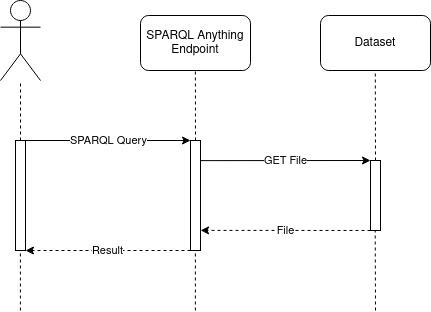
\includegraphics[width=8cm, height=6cm]{Images/UMLSequenceDiagram.drawio.png}
\end{center}
\vspace{-0.5cm}
\caption{UML Sequence Diagram}
\end{figure}
\vspace{-0.7cm}

\section{Ontology Structure}
\hspace{0.5cm} In this section, a plan for the ontology's general structure will be outlined based on: the dataset, provided ontology and any external websites. Relevant relationships to be used in the real ontology will also be noted. 

\begin{figure}[H]
    \begin{center}
        \begin{tikzpicture} [
            circle/.style={draw=blue, ellipse, ultra thick, fill=blue!30},
            align=center,
            node distance=2.5cm ]
            
        \node[circle] (q0) {organ};
        \node[circle, right of=q0, xshift=2.5cm] (q1)  {technical} ;
        \node[circle, left of=q0, xshift=-2.5cm] (q2)  {changes};
        \node[circle, above of=q0] (q3)  {disposition};
        \node[circle, below of=q0] (q4)  {organWikidata};
    
        \draw[] (q0.east) -- (q1.west) node [midway, fill=white] {xyz:technicals};
        \draw[] (q0.west) -- (q2.east) node [midway, fill=white] {xyz:changes};
        \draw[] (q0.north) -- (q3.south) node [midway, fill=white] {xyz:disposition};
        \draw[] (q0.south) -- (q4.north) node [midway, fill=white] {oont:extraInformation };
            
        \end{tikzpicture}
    \end{center}
    \vspace{-0.4cm}
\caption{Core Organ Ontology}
\end{figure}
\vspace{-0.1cm}

\textit{Figure 7.2} illustrates the main components to be expanded upon in the ontology based on data in the dataset. More details of the main nodes are detailed below:

\vspace{-0.1cm}
\begin{itemize}
    \item \textbf{organ}: \vspace{-0.075cm}\\ The primary organ component that will connect with other many other nodes.
    \vspace{-0.15cm}
    \item \textbf{changes}:\vspace{-0.075cm}\\ This component specifies the organ adjustment details and maintenance changes for an organ.
    \vspace{-0.15cm}
    \item \textbf{disposition}:\vspace{-0.075cm}\\ This component refers to the organ's current components and details relating to them.
    \vspace{-0.15cm}
    \item \textbf{technicals}: \vspace{-0.075cm}\\This component is responsible for the specific musical details of the organ. 
    \vspace{-0.15cm}
    \item \textbf{organWikidata}:\vspace{-0.075cm} \\This provides an expansion point from Wikidata for the existing knowledge graph.
\end{itemize}

The section of the ontology specifically for external Wikidata links can be structured in the same format as displayed on its website. Using \textit{Figure 7.2}, extending the \textit{organWikidata} node is most plausible. For instance, the organ page on Wikidata \cite{organwikidata} contains organ-related triples. An extract from \cite{organwikidata} is shown below:

\lstset
{
    breaklines=true,
    breakatwhitespace=true,
    basicstyle=\linespread{1.5}\ttfamily,
}
\begin{lstlisting}
organ subclassOf keyboardInstrument
organ subclassOf buildingComponent
organ studiedBy organology 
...
\end{lstlisting}

In this case, `organ' can be replaced with our \textit{organWikidata} node and the corresponding relationships and objects will be added to the ontology. All the extra nodes and edges can be added as external links to the knowledge graph using their unique Wikidata URI. 

\section{Query Flow Diagram}
\hspace{0.5cm} A flow diagram is a graphical representation of the sequence of steps or actions that need to be taken to complete a process \cite{flowchart}.

In this section, the logic required to build the SPARQL Anything Query will be illustrated in the form of a flow diagram. This will provide the structure required to build the query and produce a knowledge graph.

\begin{figure}[H]
    \begin{center}
        \begin{tikzpicture} [
            circle/.style={draw=green, ellipse, ultra thick, fill=green!30},
            align=center,
            node distance=2.5cm ]
        \node[circle] (q0) {1. Add ontology};
        \node[circle, below of=q0] (q1)  {2. Query dataset};
        \node[circle, below of=q1] (q2)  {3. Clean \& create data path};
        \node[circle, below of=q2] (q3)  {4. Retrieve data from dataset};
        \node[circle, below of=q3] (q4)  {5. Add to Knowledge Graph};
        \node[circle, below of=q4] (q5)  {6. Clean \& create external link};
        \node[circle, below of=q5] (q6)  {7. Add to Knowledge Graph};
        \node[circle, below of=q6] (q7)  {8. Add any other external links};
        \node[circle, below of=q7] (q8)  {9. Output Knowledge Graph};
    
        \draw[->] (q0.south) -- (q1.north);
        \draw[->] (q1.south) -- (q2.north);
        \draw[->] (q2.south) -- (q3.north) node [midway, fill=white] {Using cleaned data};
        \draw[->] (q3.south) -- (q4.north);
        \draw[->] (q4.south) -- (q5.north);
        \draw[->] (q5.south) -- (q6.north);
        \draw[->] (q6.south) -- (q7.north);
        \draw[->] (q7.south) -- (q8.north);
        \draw[->] (q4.east) to [out=0,in=0] (q1.east);
        \draw[->] (q4.east) to [out=0,in=0] (q7.east);
        \draw[->] (q6.west) to [out=180,in=180] (q1.west);
    
        \end{tikzpicture}
    \end{center}
    \vspace{-0.4cm}
    \caption{Query Flow Diagram}
\end{figure}
\vspace{-0.1cm}

The nodes in \textit{Figure 7.3} represent necessary actions and one of the edges is explicitly stated for clarity. Below, an explanation for each node is provided: 

\begin{enumerate}
  \item \textbf{`Add ontology' node} \\ Adds ontology to the CONSTRUCT clause of the query.
  \item \textbf{`Query dataset' node} \\ Uses SPARQL Anything to specify the file containing data of interest.
  \item \textbf{`Clean \& create data path' node} \\ Uses string manipulation to create a valid path to desired data in the dataset. 
  \item \textbf{`Retrieve data from dataset' node} \\ Uses created path above to retrieve correct data.
  \item \textbf{`Add to knowledge graph' node} \\ Adds retrieved data to the knowledge graph. Then, it either loops to step 2 using a different JSON file, continues to step 6 by adding custom external links or skips to step 8 to add other independent external links. The latter pertains to the last SPARQL Anything call in the query. 
  \item \textbf{`Create \& clean external link' node} \\ Creates an external link using retrieved data within the same SPARQL Anything call.
  \item \textbf{`Add to knowledge graph' node} \\ Adds the custom external link to the knowledge graph. Then, it either loops to step 2 using a different JSON file or continues to step 8 to add other independent external links. The latter pertains to the last SPARQL Anything call in the query. 
  \item \textbf{`Add any other external links' node} \\ Adds any other links that do not require data from the dataset such as Wikidata and MusicBrainz.
  \item \textbf{`Output knowledge graph' node} \\ Produces the resulting knowledge graph.
\end{enumerate}

\section{Query Skeleton Structure}
\hspace{0.5cm} In this section, the flow diagram illustrated in \textit{section 7.3} will be used to structure the query and aid in generating a knowledge graph. This can be observed in the comments next to each line, which correspond to a step in the flow diagram created. It also outlines the basic structure that will be used to create the query.

\lstset
{
    breaklines=true,
    breakatwhitespace=true,
    basicstyle=\linespread{1.25}\ttfamily,
}
\begin{lstlisting} 
PREFIX ... # Add relevant links

CONSTRUCT {
    ... # Add organ ontology
} 
WHERE 
    { 
        SERVICE <x-sparql-anything:file:./___.json>  # Query dataset
        { 
            ... # Clean and create data path
            ... # Retrieve data from dataset
            ... # Add to Knowledge Graph
            ... # Clean and create external link (if applicable)
            ... # Add to Knowledge Graph
        } 
        SERVICE <x-sparql-anything:file:./___`.json>  # Query dataset
        { 
            ... # Clean and create data path
            ... # Retrieve data from dataset
            ... # Add to Knowledge Graph
            ... # Clean and create external link (if applicable)
            ... # Add to Knowledge Graph
        } 
        .
        .
        .
        ... # Add any other external links 
        # Output Knowledge Graph
    }
}
\end{lstlisting}

With regard to \textit{Figure 7.3}, the query skeleton structure abides by the plan set out. Below, a small description mapping each node in \textit{Figure 7.3} will be provided.

\begin{itemize}
    \item \textbf{Add relevant links} \\ Will add any PREFIXES necessary during implementation. 
    \item \textbf{Add organ ontology} \\  Refers to node 1, where the ontology is adjusted if necessary and placed into the query's CONSTRUCT clause. 
    \item \textbf{Query Dataset} \\ Refers to node 2 by selecting the file in the dataset where desired data resides by overriding SPARQL's SERVICE operator.
    \item \textbf{Clean \& create data path} \\ Refers to node 3 and uses SPARQL 1.1 functions such as CONCAT and BIND to create the appropriate JSON path. 
    \item \textbf{Retrieve data from dataset} \\ Refers to node 4 whereby data is located using fx:properties and the recently created JSON path. 
    \item \textbf{Add to knowledge graph} \\ Refers to node 5 and adds located data to the knowledge graph using RDF functioning. Possible directions for continuation have been detailed in \textit{Section 7.3}.
    \item \textit{Optional}: \textbf{Clean \& create external link} \\ Refers to node 6 and uses SPARQL 1.1 functions such as CONCAT, IRI, REPLACE and BIND to create the external link.
    \item  \textit{Optional}: \textbf{Add to knowledge graph} \\ Refers to node 7 where located data is added to the knowledge graph by assigning it to the corresponding variable in the ontology. Possible directions for continuation have been detailed in \textit{Section 7.3}.
    \item \textbf{Add any other external links} \\ Refers to node 8 which ceases SPARQL Anything calls and adds any relevant external links using SPARQL's BIND function. Explicitly stating the links and adding them to the knowledge graph may be a viable method. 
    \item \textbf{Output Knowledge Graph} \\ Refers to node 9 where the final knowledge graph is produced. 
\end{itemize}

\chapter{Implementation}
This chapter will detail the implementation phase of the project and how the solution was reached using the design section and following the specification. 

\section{Command Line Command}
\hspace*{0.5cm} Before starting implementation, familiarisation of command line commands is necessary to understand in order to commence implementation. Since the executable .jar file enables anyone to use SPARQL-Anything, starting the command with the execution of the .jar file is needed. For example:

\lstset
{
    breaklines=true,
    breakatwhitespace=true,
    basicstyle=\ttfamily,
}
\begin{lstlisting}
    java -jar sparql-anything-0.8.0.jar 
\end{lstlisting}

\noindent Then, expand it to specify the file that contains the query by specifying it's location. For example:

\lstset
{
    breaklines=true,
    breakatwhitespace=true,
    basicstyle=\ttfamily,
}
\begin{lstlisting}
    -q filepath/filename.sparql
\end{lstlisting}

\noindent Because the project involves generating a knowledge graph of the user's choice, passing a parameter into the query is vital. It can be done as follows: 

\lstset
{
    breaklines=true,
    breakatwhitespace=true,
    basicstyle=\ttfamily,
}
\begin{lstlisting}
    --values variable=variablevalue
\end{lstlisting}

\noindent The assigned variable can be used in the SPARQL query by specifying the variable name by adding a question mark and underscore at the front. So passing the parameter 'variable', following the previous example, can be accessed using:

\lstset
{
    breaklines=true,
    breakatwhitespace=true,
    basicstyle=\ttfamily,
}
\begin{lstlisting}
    ?_variable
\end{lstlisting}

\noindent If necessary, the resulting knowledge graph can be output into a file given a folder location. For example:

\lstset
{
    breaklines=true,
    breakatwhitespace=true,
    basicstyle=\ttfamily,
}
\begin{lstlisting}
    --output filepath/outptufile.ttl
\end{lstlisting}

\noindent Altogether, the command will look like this:

\lstset
{
    breaklines=true,
    breakatwhitespace=true,
    basicstyle=\ttfamily,
}
\begin{lstlisting}
    java -jar sparql-anything-0.8.0.jar
    -q filepath/filename.sparql --values variable=variablevalue --output filepath/outptufile.ttl
\end{lstlisting}

\noindent In English, this command states: \\
\hspace*{0.5cm} "Using the executable file sparql-anything-0.8.0.jar, execute the query in filename.sparql from the filepath folder and pass in variable into the query with value variablevalue and output the knowledge in outputfile.ttl from the same filepath". 

\section{Prefixes}
\hspace*{0.5cm} The prefixes used in the ontology are mainly used in the relationship part of the triples. Below are the PREFIX that will be used:

\lstset
{
    breaklines=true,
    breakatwhitespace=true,
    basicstyle=\ttfamily,
}
\begin{lstlisting}
    PREFIX rdf:  <http://www.w3.org/1999/02/22-rdf-syntax-ns#>
    PREFIX rdfs: <http://www.w3.org/2000/01/rdf-schema#>
    PREFIX fx:   <http://sparql.xyz/facade-x/ns/>
    PREFIX xyz:  <http://sparql.xyz/facade-x/data/>
    PREFIX oont: <http://w3id.org/polifonia/ontology/organs/>
    PREFIX wd: <https://www.wikidata.org/wiki/> 
\end{lstlisting}

\section{Ontology Reconstruction}
\hspace*{0.5cm} As mentioned in the design, the scope of the provided ontology was too broad for the envisioned knowledge graph. Therefore, refinement of the provided ontology and exploration with external links was necessary to produce a relevant ontology. In the following subsections, the process of creating the ontology using the dataset and external data will be detailed. This ontology will be input into the CONSTRUCT segment of the query which acts as the framework for the knowledge graph as mentioned in the context chapter. 

\subsection{Dataset Ontology}
\hspace*{0.5cm} Using \textit{Figure 7.1}, identification and grouping of relevant data to create a more expansive ontology. 

\subsubsection{Organ}
\hspace*{0.5cm} After selecting the most relevant information to the organ from each of the .json files that stores the data, it was attached to the organ node. Using the provided ontology to identify data relevant to the organ node was used as well to ensure the correct relationships were stated. Relevant data and relationship to the organ are listed below:

\begin{itemize}
    \itemsep0em 
    \item \textit{technicals} - xyz:technicals
    \item \textit{disposition} - xyz:disposition
    \item \textit{change} - xyz:change
    \item builder - oont:builder
    \item originalLocation - oont:consolelocation
    \item dateOfBirth - oont:dateOfBirth
    \item building - oont:monument
    \item monumentNumber - oont:monumentNumber
    \item organName - oont:name
    \item organNumber - oont:organNumber 
    \item state - oont:state 
    \item particularity - oont:particularities
    \item history - oont:history
    \item creator - oont:creator
    \item moreInformation - oont:moreInformation 
\end{itemize}

This data is directly relevant to the organ as illustrated in the provided organ ontology. Data such as originalLocation, dateOfbirth and state were added as they were part of the dataset and relevant to the organ. Because technicals, disposition and change were identified as nodes for further expansion, they were connected to the main organ node. 

The relationships used to describe the relation between the organ and it's objects were provided and usually had intuitive names usually based on the object. 

\subsubsection{Technicals}
\hspace*{0.5cm} This branch of technical data regarding the organ was mainly derived off one .json file and the section of the provided ontology that referred to it's 'parthood'. All relationships branching from this 'technicals' node were provided. Relevnat data and relationships identified are below:

\begin{itemize}
    \itemsep0em 
    \item systemPlayingAids - oont:systemPlayingAids
    \item pitch - oont:pitch
    \item range1 -  oont:keyboardRange
    \item range2 - oont:pedalRange
    \item temperature - oont:temperature
    \item windPressure - oont:windPressure
    \item windSystem - oont:windSystem
\end{itemize}

\textit{range1} and \textit{range2} corresponded to the ranges of the keyboard and pedal respectively so their relationship noted it as such. 

\subsubsection{Disposition}
\hspace*{0.5cm} This branch of data referred to the qualities of the selected organ. The provided ontology covered this section but had nodes that did not appear in the dataset so needed to be adjusted. Relationships were also provided. The readjustment of the ontology would include:

\begin{itemize}
    \itemsep0em 
    \item divisionName - xyz:divisionName
    \item partition - oont:partition
    \item specification - oont:AdditionalSpecification
\end{itemize}

\subsubsection{Change}
\hspace*{0.5cm} This branch stated the changes made to the organ during it's lifetime. The provided ontology did not mention changes of a given organ so it was added to represent it from the dataset into the knowledge graph. The relationships used were provided. The new section added to the ontology were:

\begin{itemize}
    \itemsep0em 
    \item dateChange - oont:date 
    \item description - oont:AdditionalSpecification
    \item maintainer - oont:Builder
\end{itemize}

\subsection{External Ontology}
\hspace*{0.5cm} The method in which external data will be added to the knowledge graph will involve \textit{Figure 7.2}.

\subsubsection{External Data Sources}
\hspace*{0.5cm} As mentioned in the specification section, Wikidata and MusicBrainz can be used to expand the existing knowledge graph. Following the design created, a node branching out of the main organ node was made to represent Wikidata's organ page \cite{organwikidata} from which the same structure was employed. The relationships used were the same as those on Wikidata. The data branching off the organwikidata node with their corresponding relationship were:

\begin{itemize}
    \itemsep0em 
    \item keyboardinstrument - wd:Property:P279
    \item buildingcomponent - wd:Property:P279
    \item organology - wd:Property:P2579 
    \item westernclassicalmusic - wd:Property:P366
    \item musictradition - wd:Property:P366
    \item organexpert - wd:Property:P3095
    \item organist - wd:Property:P1535
    \item catholicencyclopedia - wd:Property:P1343
    \item metropolitanmuseumofarttaggingvocabulary - wd:Property:P1343
    \item dbpedia - wd:Property:P1709
    \item organcase - wd:Property:P527
    \item organpipe - wd:Property:P527
    \item musicalkeyboard - wd:Property:P527
    \item pedalkeyboard - wd:Property:P527
    \item organstop - wd:Property:P527
    \item organconsole - wd:Property:P527
    \item swellbox - wd:Property:P527
    \item pipeorgan - wd:Property:P1889
\end{itemize}

The external data from MusicBrainz's organ page \cite{organmusicbrainz} was not as vast but extended the knowledge graph in a different way to Wikidata with overlapping data being connected. Expanding from the main organ node using relationships defined on MusicBrainz, provided more context with the relationships mirroring that of MusicBrainz as well. This can be seen below:

\begin{itemize}
    \itemsep0em 
    \item barrelorgan - rdfs:subclassOf
    \item electricorgan - rdfs:subclassOf
    \item pipeorgan - rdfs:subclassOf
    \begin{itemize}
        \itemsep0em 
        \item pipeorganinfo - oont:extraInformation
    \end{itemize}
    \item reedorgan - rdfs:subclassOf
    \begin{itemize}
        \itemsep0em 
        \item reedorganimage - oont:locationImage
    \end{itemize}
    \item windinstrument - rdf:type
    \item organwikidata - 
\end{itemize}

\subsubsection{Custom Links}
\hspace*{0.5cm} These links used data from the dataset to form custom links, using string manipulation, as points of expansion. Identifying data from the dataset that was able to be expanded upon was difficult as data was very specific to the organ and external links online were too broad. However, data in the dataset that was more general such as locations could be expanded upon. Some points of expansion are:

\begin{itemize}
    \itemsep0em 
    \item buildinginfo
    \item stateinfo
    \item maintainerinfo
\end{itemize}

The relationship for all additional nodes is "oont:extraInformation".

\subsubsection{Generic Links}
\hspace*{0.5cm} These links are not organ-specific but provide more detail and general information regarding some aspects of the knowledge graph. The data in the dataset being so specific hinders the amount of external generic links that can be added, nevertheless, there are some points of expansion such as:

\begin{itemize}
    \itemsep0em 
    \item pitchinfo
    \item windPressureInfo
    \item divisionInfo
\end{itemize}

The relationship for all additional nodes is "oont:extraInformation".

\subsection{Final Ontology}
\hspace*{0.5cm} Combining both dataset and external data to form one ontology can be seen in RDF. This ontology can be placed in the CONSTRUCT section of the query.

\section{Knowledge Graph Generation}
\hspace*{0.5cm} The process of creating the knowledge graph generation query for the ontology will be detailed below:

\subsection{Dataset Knowledge Graph Query}
\hspace*{0.5cm} This subsection will detail the process for creating the query that is responsible for extracting data from the dataset using \textit{Figure 7.2} and query skeleton structure in the design section. All code in this section will be part of the WHERE clause of the query. Below is an example of data abstraction from a .json file:

\lstset
{
    breaklines=true,
    breakatwhitespace=true,
    basicstyle=\ttfamily,
}
\begin{lstlisting}
    SERVICE <x-sparql-anything:file:./output/history_base.json> 
    {
    BIND(CONCAT("$.", ?_organ, ".originallocation") AS ?organOriginalLocation) .

    fx:properties
        fx:json.path.1 ?organOriginalLocation ; .

    [] a fx:root; 
        rdf:_1 ?originalLocation ;
    } 
\end{lstlisting}

The snippet above follows \textit{Figure 7.2} and is the same structure of most SPARQL-Anything SERVICE calls in the query. 

\begin{enumerate}
    \item SERVICE call itself queries the \textit{history\_base.json} file in the \textit{output} folder using SPARQL-Anything. 
    \item BIND creates the JSON path using the parameter \textit{?\_organ} which was passed in through the command line, so the correct data can be found for the right organ. 
    \item \textit{fx:properties} then locates the data, which is assigned to the variable \textit{?originalLocation}. 
    \item ?originalLocation is used and added to the knowledge graph.
\end{enumerate}

This SPARQL-Anything call is followed by many other SPARQL-Anything calls to complete the knowledge graph. Although not explicitly stated in the design, the passed in organ \textit{?\_organ} is bound to the ontology variable \textit{?organ} in the first SPARQL-Anything call as seen below:

\lstset
{
    breaklines=true,
    breakatwhitespace=true,
    basicstyle=\ttfamily,
}
\begin{lstlisting}
    BIND (?_organ AS ?organ) .
\end{lstlisting}

\subsection{External Knowledge Graph Query}
\hspace*{0.5cm} This subsection will describe the process in which external data was added to the knowledge graph and how it was implemented in the query. 

\subsubsection{Custom Data}
\hspace*{0.5cm} For links that required data from the dataset, the query skeleton structure and \textit{Figure 7.2} was followed providing the framework to create the query. Custom links were created from Wikipedia as it was one of the few websites that covered the scope of what could be added. It also gave adequate extra information for the data and sufficiently extended the breadth of the resulting knowledge graph. To match the context of the dataset, the link created was from the Dutch version of Wikipedia. As mentioned in the ontology creation section, custom links were difficult to identify using the dataset as data was very specific to a particular organ. An example of a custom link addition can be seen below:

\lstset
{
    breaklines=true,
    breakatwhitespace=true,
    basicstyle=\ttfamily,
}
\begin{lstlisting}
    SERVICE <x-sparql-anything:file:./output/base.json>
    {
        BIND(CONCAT("$.", ?_organ, ".building") AS ?organBuilding) .
    
        fx:properties
            fx:json.path.1 ?organBuilding ; .
    
        [] a fx:root; 
            rdf:_1 ?building ;
    
        BIND(IRI(REPLACE(CONCAT("https://nl.wikipedia.org/wiki/", ?building), " ", "_")) AS ?buildingInfo) . 
    } 
\end{lstlisting}

The snippet above also follows \textit{Figure 7.2} and is used whenever a custom external link is added to the knowledge graph. The beginning of the query follows the same format as the dataset knowledge graph query but has an extra line at the end.

Using string manipulation and other SPARQL functions, the custom link is created as follows:
\begin{enumerate}
    \item \textbf{CONCAT} combines the building name retrieved from the dataset (stored in the \textit{?\_building} variable) with a generic Dutch Wikipedia link.
    \item \textbf{REPLACE} removes spaces in the \textit{?\_building} variable (if any) and replaces them with underscores to create a valid link. 
    \item \textbf{IRI} takes this new string and converts it into a URI.
    \item \textbf{BIND} takes this newly created link and assigns it to the variable \textit{?buildingInfo} to be added to the knowledge graph. 
\end{enumerate}

This is an example of where SPARQL-Anything's Facade-X approach is useful because  features of SPARQL within a SPARQL-Anything query can be used without having to learn something completely new. 

\subsubsection{General Data}
\hspace*{0.5cm} For links that were independent of the dataset, they were added after the SPARQL-Anything calls to stay consistent with \textit{Figure 7.2}. For the links personally identified, they were added with the corresponding node which they expanded upon. These specific links were found for data that had a broad scope, so websites regarding those subjects could be found. For example:

\lstset
{
    breaklines=true,
    breakatwhitespace=true,
    basicstyle=\ttfamily,
}
\begin{lstlisting}
SERVICE <x-sparql-anything:file:./output/tech.json>
{
    BIND(CONCAT("$.", ?_organ, ".pitch") AS ?organPitch) .

    fx:properties
        fx:json.path.1 ?organPitch ; .

    [] a fx:root; 
        rdf:_1 ?pitch ;
    
    BIND(URI("https://organhistoricalsociety.org/OrganHistory/works/works04.htm") AS ?pitchInfo) .
} 
\end{lstlisting}

This snippet follows the same structure as most SPARQL-Anything calls, but the last line binds the URI to \textit{?pitchInfo}. This website was found particularly to find more information describing the pitch of an organ. 

External data regarding MusicBrainz and Wikidata were added by following the format on the website and bound to a variable in the ontology. Most data on the website used links from Wikidata so the PREFIX \textit{wd} (for Wikidata was used), but some had explicit links. For example:

\lstset
{
    breaklines=true,
    breakatwhitespace=true,
    basicstyle=\ttfamily,
}
\begin{lstlisting}
    BIND(wd:Q752638 AS ?barrelOrgan) . 
    BIND(IRI("https://dbpedia.org/ontology/Organ") AS ?dbpedia) .
\end{lstlisting}

\subsection{Final Knowledge Graph Query}
\hspace*{0.5cm} The final query to generate the knowledge graph involves: 

\begin{enumerate}
    \item CONSTRUCT: Ontology
    \item WHERE:
    \begin{enumerate}
        \item SERVICE: call to SPARQL-Anything
        \item External Data
    \end{enumerate}
\end{enumerate}

% Testing based on requirements & specification

\chapter{Evaluation}
This chapter details how the knowledge graph is evaluated upon completion and measures implementation success. Both qualitative and quantitative methods were used during this section to provide a comprehensive evaluation.

\section{Requirements-Based Assessment}
\hspace{0.5cm} Assessing whether the requirements listed in the \textit{Requirements} chapter were achieved is important to measure success of implementation. For each requirement, a description stating whether it was achieved will be provided. 

\subsection{Software Requirement Assessment}
\begin{longtable}{|p{2.25cm}|p{5.5cm}|p{5.5cm}|}

\hline
\textbf{Requirement No.} & \textbf{Software Requirement} & \textbf{Assessment}\\
\hline

1& 
Ontology must be correctly configured and input into SPARQL-Anything CONSTRUCT &
Ontology has been refined and adapted based on the needs of the project. All relationships or triples have either been derived from the provided ontology or appended to the ontology based on the dataset. \\
\hline

2&
The knowledge graph created must correctly reflect the organ dataset and follow ontology structure. &
Knowledge graph produced does reflect data from the organ dataset. More detail on the quality of the knowledge graph is in the next section. \\
\hline

3&
The dataset must be refined to ensure correct data is being input into the knowledge graph. &
Query correctly extracts the correct data from the dataset and adds it onto the knowledge graph. Data is usually mapped onto the ontology one-to-one, without further adjustment to ensure correct data is input into the knowledge graph. \\
\hline

4&
The knowledge graph must expand on the current dataset using external links. &
Using the organ Wikidata site \cite{organwikidata} and organ MusicBrainz site \cite{organmusicbrainz}, data was added to the existing knowledge graph. Custom links based on data in the dataset as well as other external links were also added as extensions to the knowledge graph. \\
\hline

5&
Knowledge graphs must be evaluated to prove correctness and validity. &
This will be evaluated in the next section: \textit{Knowledge Graph Assessment Quality} \\ 
\hline

6&
Scalability of knowledge graph generation must be assessed. &
This will be assessed and evaluated in detail in the \textit{Query Scalability Assessment} section. \\ 
\hline
\caption{Software Requirement Assessment Table}
\end{longtable}

\subsection{User Requirement Assessment}

\begin{longtable}{|p{2.25cm}|p{4.5cm}|p{6.5cm}|}
\hline
\textbf{Requirement No.} & \textbf{User Requirement} & \textbf{Assessment}\\
\hline

1& 
User must be able to execute written query. &
User can download SPARQL Anything \cite{sparqlanythinggithub} and execute a given query on command line. \\
\hline

2&
User must be able to select an organ to view information on. &
User can view the codes of all available organs in the dataset. This organ code can then be passed through command line, which generates a custom knowledge graph upon execution. \\
\hline

3&
User must be able to see the knowledge graph after the query is executed. &
User can either view the knowledge graph on command line or in a .TTL file with a specified location and file name. \\
\hline

4&
User must be able to see relevant data in the knowledge graph. &
User can view the knowledge graph and see relevant data corresponding to the requested organ. \\
\hline

5&
User must be able to view other relevant external data in the knowledge graph. &
User can view the knowledge graph and see external links as well as custom links based on data from the requested organ. \\ 
\hline

\caption{User Requirement Assessment Table}
\end{longtable}
\vspace{-1.1cm}

\section{Knowledge Graph Quality Assessment}
\hspace{0.5cm} Assessment of knowledge graph quality is important to ensure the produced knowledge graph is valid and correct, using \cite{knowledgegraphevaulationbook} as guidance to assess knowledge graph quality. The 18 qualitative requirements detailed in \cite{evaluationpaper} are also used to assess quality. For each section, specific details are assessed with explanations and assessment of knowledge graph quality. 

The main three sections used to assess knowledge graph quality are: 

\vspace{-0.2cm}
\begin{itemize}
    \itemsep0em 
    \item Accuracy
    \vspace{-0.15cm}
    \item Coverage
    \vspace{-0.15cm}
    \item Succinctness
\end{itemize}
\vspace{-0.1cm}

For each section, generated knowledge graphs for five different organs will be used to measure overall quality. Organs to be tested from the dataset are: \textit{Part14\_000Brouwershaven}, \textit{Part14\_000Niezijl}, \textit{Part14\_000Folsgare}, \textit{Part14\_000GravenhageNoorderkerk} and \textit{Part14\_000Groede}. For simplicity, a random sample of five was selected from the list of organ codes and the produced knowledge graphs will represent the quality of all possible organs. Generating the knowledge graphs and assessing quality from the output files was the method employed. 

\subsection{Accuracy}
\hspace{0.5cm} ``Accuracy refers to the extent to which entities and relations- encoded by nodes and edges in the graph- correctly represent real-life phenomena". \cite{knowledgegraphevaulationbook}. In this context, accuracy means the knowledge graph generated (both subjects and relationships) needs to correctly reflect the relationships between organ topics. 

There are three types of accuracy: 

\vspace{-0.2cm}
\begin{itemize}
    \itemsep0em 
\item Syntactic Accuracy.
\vspace{-0.1cm}
\item Semantic Accuracy.
\vspace{-0.1cm}
\item Timeliness.
\end{itemize}
\vspace{-0.4cm}

\subsubsection{Syntactic Accuracy}
\hspace{0.5cm} Syntactic accuracy refers to whether the data presented is valid for its given type. \cite{knowledgegraphevaulationbook}

\noindent An example of a potential violation: 
\begin{displayquote}
    \textit{``This is an organ" would be incompatible with xsd:integer.}
\end{displayquote}

Upon assessing the produced knowledge graphs for each of the five organs, no syntactic inaccuracies were found. Checks for each organ were carried out and due to the ontology being derived from the provided ontology and external links, all resulting knowledge graphs should not, in theory, contain any syntactic inaccuracies. 

\subsubsection{Semantic Accuracy}
\hspace{0.5cm} Semantic accuracy refers to whether data values are being correctly represented in a real-world context. \cite{knowledgegraphevaulationbook}

\noindent An example of a potential violation: 
\begin{displayquote}
    \textit{Date of build (for an organ) coming after today's date.}
\end{displayquote}

In regards to semantic accuracy, none of the five organs contained semantic inaccuracies upon assessment. This can be explained for similar reasons as above regarding the lack of syntactic inaccuracies. 

\subsubsection{Timeliness}
\hspace{0.5cm} Timeliness refers to how up-to-date or relevant the knowledge graph is with the real current state of the modern world \cite{knowledgegraphevaulationbook}. This is also in line with \cite{evaluationpaper} stating that ``Knowledge graphs should contain the latest resources to guarantee freshness".

\noindent An example of a potential violation:
\begin{displayquote}
    \textit{Organ's location stated as ``Netherlands", but has recently been moved to Portugal and the knowledge graph has not been updated.}
\end{displayquote}

In the produced knowledge graphs, violations of timeliness can occur due to the static nature of the dataset. An example of a violation may occur when the \textit{?divisionName} is no longer the organ's current disposition in real life, but data in the dataset is not up-to-date. This particular violation will occur over time as the organ's divisions can change over time. However, at the current moment in time, no timeliness violations occur in the five produced knowledge graphs.

\subsection{Coverage}
\hspace{0.5cm} ``Coverage refers to avoiding the omission of domain-relevant elements, which may yield incomplete results". \cite{knowledgegraphevaulationbook}. In this context, the knowledge graph must completely fill the ontology framework in all of its nodes and edges. This is to accurately represent the entire dataset given. 

\noindent There are two types of coverage: 

\vspace{-0.15cm}
\begin{itemize}
\itemsep0em 
\item Completeness.
\vspace{-0.1cm}
\item Representativeness.
\end{itemize}
\vspace{-0.4cm}

\subsubsection{Completeness}
\hspace{0.5cm} Completeness ensures the knowledge graph is correctly filled with all the relevant information present in a particular dataset. \cite{knowledgegraphevaulationbook}. Adding contextual information about entities and from different resources \cite{evaluationpaper} is also important to ensure completeness. 

\noindent Some examples of potential violations:

\vspace{-0.15cm}
\begin{displayquote}
    \textit{- Organ classes lacking information.}
\end{displayquote}
\vspace{-0.6cm}
\begin{displayquote}
    \textit{- Important values missing for a specific organ property.}
\end{displayquote}
\vspace{-0.1cm}

With regard to dataset coverage, most of the data is represented in the knowledge graph. Reasoning for the omission of some data is related to how it can be represented in the knowledge graph without it causing confusion. For example, the specific ranges of a given organ for each keyboard or pedal are omitted due to the possible confusion it may cause when representing the keyboard and pedal ranges (\textit{?range1} and \textit{?range2}). Also, representing all that data concisely would be challenging and it may be seen as unnecessary. However, this is only relevant to some data. 

Contextual information is added in the form of descriptions and custom links in all assessed knowledge graphs. The relationship \textit{oont:extraInformation}, for instance, provides context and extra detail for a specific node. 

Different resources can be seen in the five knowledge graphs such as: Wikidata links, data from the dataset and various other website links. 

\subsubsection{Representativeness}
\hspace{0.5cm} Representativeness ensures the knowledge graph does not involve any bias and does not exclude anything relevant. \cite{knowledgegraphevaulationbook}

\noindent Some examples of potential violations: 

\vspace{-0.1cm}
\begin{displayquote}
    \textit{- Under-represent organ data from other languages.}
\end{displayquote}  
\vspace{-0.6cm}
\begin{displayquote}
     \textit{- Under-represent people (e.g. organist, owner) from a particular gender, race etc. }  
\end{displayquote}
\vspace{-0.1cm}

Violations regarding under-representation stem from the dataset provided. For example, the dataset is written in Dutch so organ data is limited to the Dutch language. With regard to the under-representation of people, anyone involved with the organ is mentioned in all five knowledge graphs such as: \textit{?maintainer} and \textit{?builder} so no violations occur in that regard.

\subsection{Succinctness}
\hspace{0.5cm} ``Succinctness refers to the inclusion of relevant content that is represented in a concise and intelligible manner." \cite{knowledgegraphevaulationbook}. In this context, it means the knowledge graph created should be easily understandable and to the point. 

\noindent There are two types of succinctness: 

\vspace{-0.15cm}
\begin{itemize}
    \itemsep0em 
\item Representational Conciseness.
\vspace{-0.1cm}
\item Understandability.
\end{itemize}
\vspace{-0.4cm}

\subsubsection{Representational Conciseness}
\hspace{0.5cm} Representational conciseness refers to the extent in which the knowledge graph content is compactly represented \cite{knowledgegraphevaulationbook}. This is consistent with requirements from \cite{evaluationpaper} including: ``triples should be concise" and ``knowledge graph does not contain redundant triples".

\noindent An example of a potential violation: 
\vspace{-0.1cm}
\begin{displayquote}
    \textit{Containing two properties that serve the same purpose i.e.}
\end{displayquote}
\vspace{-0.5cm}
\begin{displayquote}
    \textit{- Organist}
\end{displayquote}
\vspace{-0.6cm}
\begin{displayquote}
    \textit{- Organ Player}
\end{displayquote}

\begin{figure}[H]
\begin{center}
    \begin{tikzpicture} [
        square/.style={draw=yellow, rectangle, ultra thick, fill=yellow!30},
        align=center,
        node distance=5cm ]
    \node[square] (q1)  {Organist};
    \node[square, right of=q1] (q2)  {Organ Player};
    \end{tikzpicture}
\end{center}
\vspace{-0.5cm}
\caption{Representational Conciseness Violation}
\end{figure}

Each knowledge graph is created with the purpose of making them concise. Creation of the ontology structure was derived and refined from the provided ontology. \textit{Figure 7.2} in the design was made specifically to represent the data in a concise manner and avoid the inclusion of redundant data. Implementation also kept this in mind when refining the ontology. Upon assessing each of the five organs, the produced knowledge graphs contain concise content.

\subsubsection{Understandability}
\hspace{0.5cm} Understandability refers to the need for readability and ease of understanding the knowledge graph generated. \cite{knowledgegraphevaulationbook}

\noindent An example of a potential violation: 
\vspace{-0.1cm}
\begin{displayquote}
    \textit{Using property names such as Organist1, when asked to state the name of an organist (Actual name should be used instead).}
\end{displayquote}

\begin{figure}[H]
\begin{center}
    \begin{tikzpicture} [
        square/.style={draw=yellow, rectangle, ultra thick, fill=yellow!30},
        align=center,
        node distance=5cm ]
    \node[square] (q1)  {Organist1};
    \end{tikzpicture}
\end{center}
\vspace{-0.5cm}
\caption{Understandability Violation}
\end{figure}

Data in the dataset is understandable from the perspective of a Dutch reader. Given the relationships, the meaning of data can be easily inferred. However, there are some cases in the produced knowledge graphs where nodes produce an empty string ``" due to empty data in the dataset. For example, the variable \textit{?partition} in the ontology is often empty and out of the five tested organs, four of the \textit{partition}'s data is missing. 

\section{Query Scalability Assessment}
In this section, scalability of the knowledge graph will be tested. In particular, the areas being measured to assist quantification of the knowledge graph scalability are: 

\vspace{-0.1cm}
\begin{itemize}
\itemsep0cm
    \item Number of SERVICE Calls.
    \vspace{-0.1cm}
    \item Size of Files.
\end{itemize}
\vspace{-0.1cm}

For each one, measurement of scalability will be computed using the time required to execute the query on command line, which is how long it takes to generate the knowledge graph. This will make use of a command on the Windows OS called: \textit{Measure-Command} \cite{measurecommand}, which measures the time required for a command to execute. For instance, measuring the time required to generate a knowledge graph for organ: \textit{Part01\_001MIDDE} is:

\lstset
{
    breaklines=true,
    breakatwhitespace=false,
    basicstyle=\ttfamily,
}
\begin{lstlisting}
    Measure-Command{java -jar sparql-anything-0.8.0.jar -q queries/organ-details.sparql --values organ=Part01_001MIDDE -o output/output.ttl}
\end{lstlisting}

The same sample of five organs will be selected for knowledge graph generation and tests will be run on a 64-bit OS with Intel(R) Core(TM) i5-8265U CPU @ 1.60GHz 1.80 GHz and 8GB RAM. Regarding time calculation, the procedure will involve running each of the five sampled organs five times using \textit{Measure-Command}, followed by calculation of the average time per organ. Finally, the mean times for all five organs will be noted.

\subsection{Size of Files}
\hspace{0.5cm} For this test, knowledge graph generation was calculated with respect to .JSON file size (from the dataset). For testing purposes, some organs may be removed from relevant data files in order to measure the effect of file size. The five tested organs, however, will always remain in the files. This is possible since the structure of each .JSON file follows the same format as shown in the \textit{Context} section. External links were left in the query as their addition did not significantly affect results. After removing organs to test file size, the actual size of a file will be noted using a VS Code extension: \textit{filesize}. A graph plotted with cumulative file sizes against time can be seen in \textit{Figure 9.3}.

\begin{figure}[H]
\begin{center}
\begin{tikzpicture}
\begin{axis}[
    axis x line=bottom,
    axis y line=left,
    xlabel=\textit{file size (MiB)},
    ylabel=\textit{time (ms)}, ]
\addplot[smooth,blue] plot coordinates {
    (0.01,1353.7575)
    (7.498502, 1751.012)
    (11.9024, 2021.9029)
    (15.27645, 2213.0641)
    (21.8746, 2464.1894)
};
\end{axis}
\end{tikzpicture}
\end{center}
\vspace{-0.75cm}
\caption{Analysis of File Size}
\end{figure}

\textit{Figure 9.3} shows an initial linear relationship between the file size and time. This shows that the knowledge graph-generating query produced is scalable to a certain extent. It is unknown, however, how well the query will perform for much larger file sizes. 

\subsection{Number of SERVICE Calls}
\hspace{0.5cm} In this test, number of SERVICE calls within the query are tested to observe their effect on the speed of knowledge graph generation. In the implemented query, removal of SERVICE calls will be done incrementally and plotted against execution time. Measuring the number of SERVICE calls will indicate the scalability of the knowledge graph, providing insight into its capacity for expansion.

For this project, knowledge graph size will increase proportionally with the number of SERVICE calls. A mock knowledge graph was created using additional SERVICE calls that were not in the project scope and added for testing purposes to measure expandability. Data gathered from the SERVICE call was added to the mock knowledge graph. This was to account for the time taken to add data onto the knowledge graph during command execution. In this particular test, all external links in the knowledge graph were removed so as to not affect execution time. The plotted graph for number of SERVICE calls against time can be seen in \textit{Figure 9.4}.

\begin{figure}[H]
\begin{center}
\begin{tikzpicture}
\begin{axis}[
    axis x line=bottom,
    axis y line=left,
    xlabel=\textit{no. SERVICE calls},
    ylabel=\textit{time (ms)}, 
    ]
\addplot[smooth,blue] plot coordinates {
    (1, 1184.163)
    (10, 1318.7934)
    (20, 1730.7290)
    (29, 1975.1539)
    (39, 2143.491)
    (49, 2340.4259)
    (59, 2520.7234)
    (99, 3420.7116)
};
\end{axis}
\end{tikzpicture}
\end{center}
\vspace{-0.75cm}
\caption{Analysis of SERVICE Calls}
\end{figure}

After plotting the graph (\textit{Figure 9.4}) of up to 100 SERVICE calls, an initial linear relationship can be seen between variables. The expandability of the knowledge graph is possible within reason. However, this graph only plots values for up to 100 SERVICE calls so time required for extremely large amounts of SERVICE calls may differ. 


\addcontentsline{toc}{section}{Bibliography}

\bibliographystyle{plain}
\bibliography{References}

\appendix
\chapter{Extra Information}
\section{Tables, proofs, graphs, test cases, ...}
% The appendices contain information that is peripheral to the main body of the report. Information typically included in the Appendix are things like tables, proofs, graphs, test cases or any other material that would break up the theme of the text if it appeared in the body of the report. It is necessary to include your source code listings in an appendix that is separate from the body of your written report (see the information on Program Listings below).


\chapter{User Guide}
\section{Instructions}
Step-by-step instructions on how to execute the knowledge graph generation query will be detailed below:

\begin{enumerate}
    \item Download project zip file on github repository: https://github.com/lamalvin21/ThirdYearProject
    \item 
\end{enumerate}

You must provide an adequate user guide for your software. The guide should provide easily understood instructions on how to use your software. A particularly useful approach is to treat the user guide as a walk-through of a typical session, or set of sessions, which collectively display all of the features of your package. Technical details of how the package works are rarely required. Keep the guide concise and simple. The extensive use of diagrams, illustrating the package in action, can often be particularly helpful. The user guide is sometimes included as a chapter in the main body of the report, but is often better included in an appendix to the main report.

\chapter{Source Code}
\section{Declaration}
``I verify that I am the sole author of the programs contained in this folder, except where explicitly stated to the contrary''. Alvin Lam- \today

\section{Github Repository Link}
Link to Github Repository containing all relevant files including the dataset. \\
https://github.com/lamalvin21/ThirdYearProject

\section{Knowledge Graph Generation Query}
The final knowledge graph generation query is below:

\lstset
{
    breaklines=true,
    breakatwhitespace=false,
    basicstyle=\linespread{1}\ttfamily,
}
\begin{lstlisting}[caption={organ-details.sparql}]

PREFIX rdf:  <http://www.w3.org/1999/02/22-rdf-syntax-ns#>
PREFIX rdfs: <http://www.w3.org/2000/01/rdf-schema#>
PREFIX fx:   <http://sparql.xyz/facade-x/ns/>
PREFIX xyz:  <http://sparql.xyz/facade-x/data/>
PREFIX oont: <http://w3id.org/polifonia/ontology/organs/>
PREFIX wd: <https://www.wikidata.org/wiki/> 

CONSTRUCT
  {
	?organ a oont:Organ ;
		oont:builder ?builder ;
		oont:consolelocation ?originalLocation ;
		oont:dateOfBirth ?dateOfBirth ;
		oont:monument ?building ;
		oont:monumentNumber ?monumentNumber ;
		oont:name ?organName ;
		oont:organNumber ?organNumber ;
		oont:state ?state ;
		oont:particularities ?particularity ;
		oont:history ?history ;
		oont:creator ?creator ;
		oont:moreInformation ?moreInformation ;
		xyz:technicals ?technicals ; 
		xyz:disposition ?disposition ;
		xyz:change ?change ;
		.

	?technicals oont:systemPlayingAids ?systemPlayingAids .
	?technicals oont:pitch ?pitch .
	?technicals oont:keyboardRange ?range1 . 
	?technicals oont:pedalRange ?range2 . 
	?technicals oont:temperature ?temperature .
	?technicals oont:windPressure ?windPressure .
	?technicals oont:windSystem ?windSystem .
	
	?disposition xyz:divisionName ?divisionName . 
	?disposition oont:partition ?partition .
	?disposition oont:AdditionalSpecification ?specification .

	?change oont:date ?dateChange .
	?change oont:AdditionalSpecification ?changeDescription . 
	?change oont:Builder ?maintainer .

	?building oont:extraInformation ?buildingInfo .
	?state oont:extraInformation ?stateInfo .
	?maintainer oont:extraInformation ?maintainerInfo .

	?pitch oont:extraInformation ?pitchInfo .
	?windPressure oont:extraInformation ?windPressureInfo .
	?windSystem oont:extraInformation ?windPressureInfo .
	?divisionName oont:extraInformation ?divisionInfo .

	?organ rdfs:subClassOf ?barrelOrgan .
	?organ rdfs:subClassOf ?electricOrgan .
	?organ rdfs:subClassOf ?pipeOrgan .
	?organ rdfs:subClassOf ?reedOrgan .
	?organ rdf:type ?windInstrument . 

	?pipeOrgan oont:extraInformation ?pipeOrganInfo .
	?reedOrgan oont:locationImage ?reedOrganImage .
	?organ oont:extraInformation ?organWikidata .

	?organWikidata wd:Property:P279 ?keyboardInstrument .
	?organWikidata wd:Property:P279 ?buildingComponent .
	?organWikidata wd:Property:P2579 ?organology .
	?organWikidata wd:Property:P366 ?westernClassicalMusic .
	?organWikidata wd:Property:P366 ?musicTradition .
	?organWikidata wd:Property:P3095 ?organExpert .
	?organWikidata wd:Property:P1535 ?organist .
	?organWikidata wd:Property:P1343 ?catholicEncyclopedia .
	?organWikidata wd:Property:P1343 ?metropolitanMuseumOfArtTaggingVocabulary .
	?organWikidata wd:Property:P1709 ?dbpedia .

	?organWikidata wd:Property:P527 ?organCase .
	?organWikidata wd:Property:P527 ?organPipe .
	?organWikidata wd:Property:P527 ?musicalKeyboard .
	?organWikidata wd:Property:P527 ?pedalKeyboard .
	?organWikidata wd:Property:P527 ?organStop .
	?organWikidata wd:Property:P527 ?organConsole .
	?organWikidata wd:Property:P527 ?swellBox .

	?organWikidata wd:Property:P1889 ?pipeOrgan .
  }
WHERE
  { 
	SERVICE <x-sparql-anything:file:./output/history_base.json> 
	{
		BIND(CONCAT("$.", ?_organ, ".builder") AS ?organBuilder) .

		fx:properties
			fx:json.path.1 ?organBuilder ; .

		[] a fx:root; 
			rdf:_1 ?builder ; 

		BIND (?_organ AS ?organ) .
	} 
	SERVICE <x-sparql-anything:file:./output/history_base.json> 
	{
		BIND(CONCAT("$.", ?_organ, ".originallocation") AS ?organOriginalLocation) .

		fx:properties
			fx:json.path.1 ?organOriginalLocation ; .

		[] a fx:root; 
			rdf:_1 ?originalLocation ;
	} 
	SERVICE <x-sparql-anything:file:./output/history_base.json> 
	{
		BIND(CONCAT("$.", ?_organ, ".year") AS ?organDob) .

		fx:properties
			fx:json.path.1 ?organDob ; .

		[] a fx:root; 
			rdf:_1 ?dateOfBirth ;
	} 
	SERVICE <x-sparql-anything:file:./output/base.json>
	{
		BIND(CONCAT("$.", ?_organ, ".building") AS ?organBuilding) .

		fx:properties
			fx:json.path.1 ?organBuilding ; .

		[] a fx:root; 
			rdf:_1 ?building ;

		BIND(IRI(REPLACE(CONCAT("https://nl.wikipedia.org/wiki/", ?building), " ", "_")) AS ?buildingInfo) . 
	} 
	SERVICE <x-sparql-anything:file:./output/base.json>
	{
		BIND(CONCAT("$.", ?_organ, ".place") AS ?organPlace) .

		fx:properties
			fx:json.path.1 ?organPlace ; .

		[] a fx:root; 
			rdf:_1 ?state ;

		BIND(IRI(REPLACE(CONCAT("https://nl.wikipedia.org/wiki/", ?state), " ", "_")) AS ?stateInfo) .
	} 
	SERVICE <x-sparql-anything:file:./output/base.json>
	{
		BIND(CONCAT("$.", ?_organ, ".monumentnumber") AS ?organMonumentNumber) .

		fx:properties
			fx:json.path.1 ?organMonumentNumber ; .

		[] a fx:root; 
			rdf:_1 ?monumentNumber ;
	} 
	SERVICE <x-sparql-anything:file:./output/base.json>
	{
		BIND(CONCAT("$.", ?_organ, ".name") AS ?organName1) .

		fx:properties
			fx:json.path.1 ?organName1 ; .

		[] a fx:root; 
			rdf:_1 ?organName ;
	} 
	SERVICE <x-sparql-anything:file:./output/base.json>
	{
		BIND(CONCAT("$.", ?_organ, ".organnumber") AS ?organNumber1) .

		fx:properties
			fx:json.path.1 ?organNumber1 ; .

		[] a fx:root; 
			rdf:_1 ?organNumber ;
	} 
	SERVICE <x-sparql-anything:file:./output/texts_tech.json> 
	{
		BIND(CONCAT("$.", ?_organ) AS ?organTechnicals) .

		fx:properties
			fx:json.path.1 ?organTechnicals; .

		[] a fx:root; 
			rdf:_1 ?technicals ; 
	} 
	SERVICE <x-sparql-anything:file:./output/tech.json>
	{
		BIND(CONCAT("$.", ?_organ, ".pitch") AS ?organPitch) .

		fx:properties
			fx:json.path.1 ?organPitch ; .

		[] a fx:root; 
			rdf:_1 ?pitch ;
		
		BIND(URI("https://organhistoricalsociety.org/OrganHistory/works/works04.htm") AS ?pitchInfo) .
	} 
	SERVICE <x-sparql-anything:file:./output/tech.json>
	{
		BIND(CONCAT("$.", ?_organ, ".pitch") AS ?organPitch) .

		fx:properties
			fx:json.path.1 ?organPitch ; .

		[] a fx:root; 
			rdf:_1 ?pitch ;
		
		BIND(URI("https://organhistoricalsociety.org/OrganHistory/works/works04.htm") AS ?pitchinfo) .
	} 
	SERVICE <x-sparql-anything:file:./output/tech.json>
	{
		BIND(CONCAT("$.", ?_organ, ".windPres") AS ?organWindPressure) .

		fx:properties
			fx:json.path.1 ?organWindPressure ; .

		[] a fx:root; 
			rdf:_1 ?windPressure ;

		BIND(URI("https://organhistoricalsociety.org/OrganHistory/works/works06.htm") AS ?windPressureInfo) .
	} 
	SERVICE <x-sparql-anything:file:./output/tech.json>
	{
		BIND(CONCAT("$.", ?_organ, ".aids") AS ?organAids) .

		fx:properties
			fx:json.path.1 ?organAids ; .

		[] a fx:root; 
			rdf:_1 ?systemPlayingAids ;
	} 
	SERVICE <x-sparql-anything:file:./output/tech.json>
	{
		BIND(CONCAT("$.", ?_organ, ".range1") AS ?organRange1) .

		fx:properties
			fx:json.path.1 ?organRange1 ; .

		[] a fx:root; 
			rdf:_1 ?range1 ;
	} 
	SERVICE <x-sparql-anything:file:./output/tech.json>
	{
		BIND(CONCAT("$.", ?_organ, ".range2") AS ?organRange2) .

		fx:properties
			fx:json.path.1 ?organRange2 ; .

		[] a fx:root; 
			rdf:_1 ?range2 ;
	} 
	SERVICE <x-sparql-anything:file:./output/tech.json>
	{
		BIND(CONCAT("$.", ?_organ, ".temperature") AS ?organTemperature) .

		fx:properties
			fx:json.path.1 ?organTemperature ; .

		[] a fx:root; 
			rdf:_1 ?temperature ;
	} 
	SERVICE <x-sparql-anything:file:./output/tech.json>
	{
		BIND(CONCAT("$.", ?_organ, ".windSys") AS ?organWindSystem) .

		fx:properties
			fx:json.path.1 ?organWindSystem ; .

		[] a fx:root; 
			rdf:_1 ?windSystem ;
	} 
	SERVICE <x-sparql-anything:file:./output/dispositions.json>
	{
		BIND(CONCAT("$.", ?_organ, ".dispositions[?(@.current==true)].description") AS ?organDescription) .

		fx:properties
			fx:json.path.1 ?organDescription ; .

		[] a fx:root; 
			rdf:_1 ?disposition ;
	} 
	SERVICE <x-sparql-anything:file:./output/dispositions.json>
	{
		BIND(CONCAT("$.", ?_organ, ".dispositions[?(@.current==true)].disposition[0].division_name") AS ?organDivisionName) .

		fx:properties
			fx:json.path.1 ?organDivisionName ; .

		[] a fx:root; 
			rdf:_1 ?divisionName ;

		BIND(URI("https://organhistoricalsociety.org/OrganHistory/works/works05.htm") AS ?divisionInfo) .
	} 
	SERVICE <x-sparql-anything:file:./output/dispositions.json>
	{
		BIND(CONCAT("$.", ?_organ, ".dispositions[?(@.current==true)].disposition[0].stoplist[0].partition") AS ?organPartition) .

		fx:properties
			fx:json.path.1 ?organPartition ; .

		[] a fx:root; 
			rdf:_1 ?partition ;
	} 
	SERVICE <x-sparql-anything:file:./output/dispositions.json>
	{
		BIND(CONCAT("$.", ?_organ, ".dispositions[?(@.current==true)].disposition[0].stoplist[0].spec") AS ?organSpec) .

		fx:properties
			fx:json.path.1 ?organSpec ; .

		[] a fx:root; 
			rdf:_1 ?specification ;
	} 
	SERVICE <x-sparql-anything:file:./output/history_projects.json>
	{
		BIND(CONCAT("$.", ?_organ, "[0].changes[0]") AS ?organChange) .

		fx:properties
			fx:json.path.1 ?organChange ; .

		[] a fx:root; 
			rdf:_1 ?change ;
	} 
	SERVICE <x-sparql-anything:file:./output/history_projects.json>
	{
		BIND(CONCAT("$.", ?_organ, "[0].date") AS ?organDateChange) .

		fx:properties
			fx:json.path.1 ?organDateChange ; .

		[] a fx:root; 
			rdf:_1 ?dateChange ;
	} 
	SERVICE <x-sparql-anything:file:./output/history_projects.json>
	{
		BIND(CONCAT("$.", ?_organ, "[0].description") AS ?organChangeDescription) .

		fx:properties
			fx:json.path.1 ?organChangeDescription ; .

		[] a fx:root; 
			rdf:_1 ?changeDescription ;
	} 
	SERVICE <x-sparql-anything:file:./output/history_projects.json>
	{
		BIND(CONCAT("$.", ?_organ, "[0].name") AS ?organMaintainer) .

		fx:properties
			fx:json.path.1 ?organMaintainer ; .

		[] a fx:root; 
			rdf:_1 ?maintainer ;

		BIND(IRI(REPLACE(CONCAT("https://nl.wikipedia.org/wiki/", ?maintainer), " ", "_")) AS ?maintainerInfo) .
	}
	SERVICE <x-sparql-anything:file:./output/texts_bijzonderheden.json> 
	{
		BIND(CONCAT("$.", ?_organ) AS ?organParticularity) .

		fx:properties
			fx:json.path.1 ?organParticularity; .

		[] a fx:root; 
			rdf:_1 ?particularity ; 
	} 
	SERVICE <x-sparql-anything:file:./output/texts_hist.json> 
	{
		BIND(CONCAT("$.", ?_organ) AS ?organHistory) .

		fx:properties
			fx:json.path.1 ?organHistory; .

		[] a fx:root; 
			rdf:_1 ?history ; 
	}
	SERVICE <x-sparql-anything:file:./output/texts_kunst.json> 
	{
		BIND(CONCAT("$.", ?_organ) AS ?organCreator) .

		fx:properties
			fx:json.path.1 ?organCreator; .

		[] a fx:root; 
			rdf:_1 ?creator ; 
	} 
	SERVICE <x-sparql-anything:file:./output/texts_lit.json> 
	{
		BIND(CONCAT("$.", ?_organ) AS ?organMoreInformation) .

		fx:properties
			fx:json.path.1 ?organMoreInformation; .

		[] a fx:root; 
			rdf:_1 ?moreInformation ; 
	}

	BIND(wd:Q752638 AS ?barrelOrgan) .
	BIND(wd:Q1327327 AS ?electricOrgan) .
	BIND(wd:Q281460 AS ?pipeOrgan) .
	BIND(IRI("https://en.wikisource.org/wiki/1911_Encyclopædia_Britannica/Organ ") AS ?pipeOrganInfo) .
	BIND(wd:Q12460259 AS ?reedOrgan) .
	BIND(IRI("https://staticbrainz.org/irombook/reed_organ/reed_organ.png") AS ?reedOrganImage) . 
	BIND(wd:Q173453 AS ?windInstrument) .
	BIND(wd:Q1444 AS ?organWikidata) .

	BIND(wd:Q52954 AS ?keyboardInstrument) .
	BIND(wd:Q19603939 AS ?buildingComponent) .
	BIND(wd:Q11163731 AS ?organology) .
	BIND(wd:Q9730 AS ?westernClassicalMusic) .
	BIND(wd:Q60733114 AS ?musicTradition) .
	BIND(wd:Q1495811 AS ?organExpert) .
	BIND(wd:Q765778 AS ?organist) .
	BIND(wd:Q302556 AS ?catholicEncyclopedia) .
	BIND(wd:Q106727050 AS ?metropolitanMuseumOfArtTaggingVocabulary) .
	BIND(IRI("https://dbpedia.org/ontology/Organ") AS ?dbpedia) .
	BIND(wd:Q2927648 AS ?organCase) .
	BIND(wd:Q1510738 AS ?organPipe) .
	BIND(wd:Q901207 AS ?musicalKeyboard) .
	BIND(wd:Q1758965 AS ?pedalKeyboard) .
	BIND(wd:Q1446290 AS ?organStop) .
	BIND(wd:Q392573 AS ?organConsole) .
	BIND(wd:Q25112583 AS ?swellBox) .
  }
\end{lstlisting}


\end{document}
